\documentclass{standalone}
\usepackage{tikz}

\begin{document}

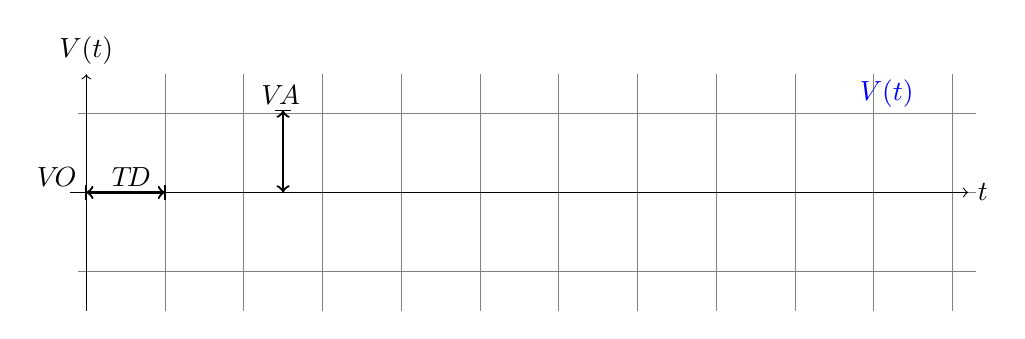
\begin{tikzpicture}[domain=0:11]
    %axes
    \draw[very thin,color=gray] (-0.1,-1.5) grid (11.3,1.5);
    \draw[->] (-0.2,0) -- (11.2,0) node[right] {$t$};
    \draw[->] (0,-1.5) -- (0,1.5) node[above] {$V(t)$};
    % the time function
    \draw[color=blue, semithick] plot[id=fm, samples=1000]
        function{(sin((x-1)*2*pi*5 + 10*sin((x-1)*2*pi/3)))*(x>=1 ? 1 : 0)} 
        node[right] {};
    % the delay TD
    \draw[semithick, -] (0,-.1) -- (0,.1) node[] {};
    \draw[semithick, -] (1,-.1) -- (1,.1) node[] {};
    \draw[thick, <->] (0,0) -- (1,0) node[] {};
    \draw[] (.2,.2) node[right] {$T\!D$};
    % the amplitude VA
    \draw[semithick, -] (2.4,0) -- (2.6,0) node[] {};
    \draw[semithick, -] (2.4,1.04) -- (2.6,1.04) node[] {};
    \draw[thick, <->] (2.5,0) -- (2.5,1.04) node[] {};
    \draw[] (2.1,1.24) node[right] {$V\!A$};
    % no offset
    \draw[] (0,.2) node[left] {$V\!O$};
    \draw[color=blue] (9.7,1.25) node[right] {$V(t)$};

\end{tikzpicture}

\end{document}
